
\subsection{Plotting of travel times, TTPLOT} 
\label{subs:ttplot}
\index{TTPLOT}

Program to plot observed and calculated travel times (Figure 
\ref{fig:travel-time-plot}
). The input to the program is an s-file, which has an indicator to a model file (\texttt{STATION?.HYP}) and the travel time observations. The program is started by `ttplot $<$sfile-name$>$'. At the start, TTPLOT relocates the event and calculates distances using the HYPOCENTER program. It then plots all observations with a `+' symbol and the theoretical travel times that are calculated by the program for the first P and S arrivals with solid lines. The program can be useful in routine processing to visualize large residuals, which otherwise are seen from the location program output. The program can also be started from EEV using option `ttplot'. It is possible to click on symbols, which will bring up station code, phase, observed travel time and residual on the rigth. The output files are: 

\texttt{ttplot.out} - gives station code, phase name, distance, observed travel times and residual. 
\newline
\texttt{ttplot.eps} -  Postscript version of plot. \index{ttplot.out}\index{ttplot.eps} 

\begin{figure}
\htmlimage{scale=2.0}
\centerline{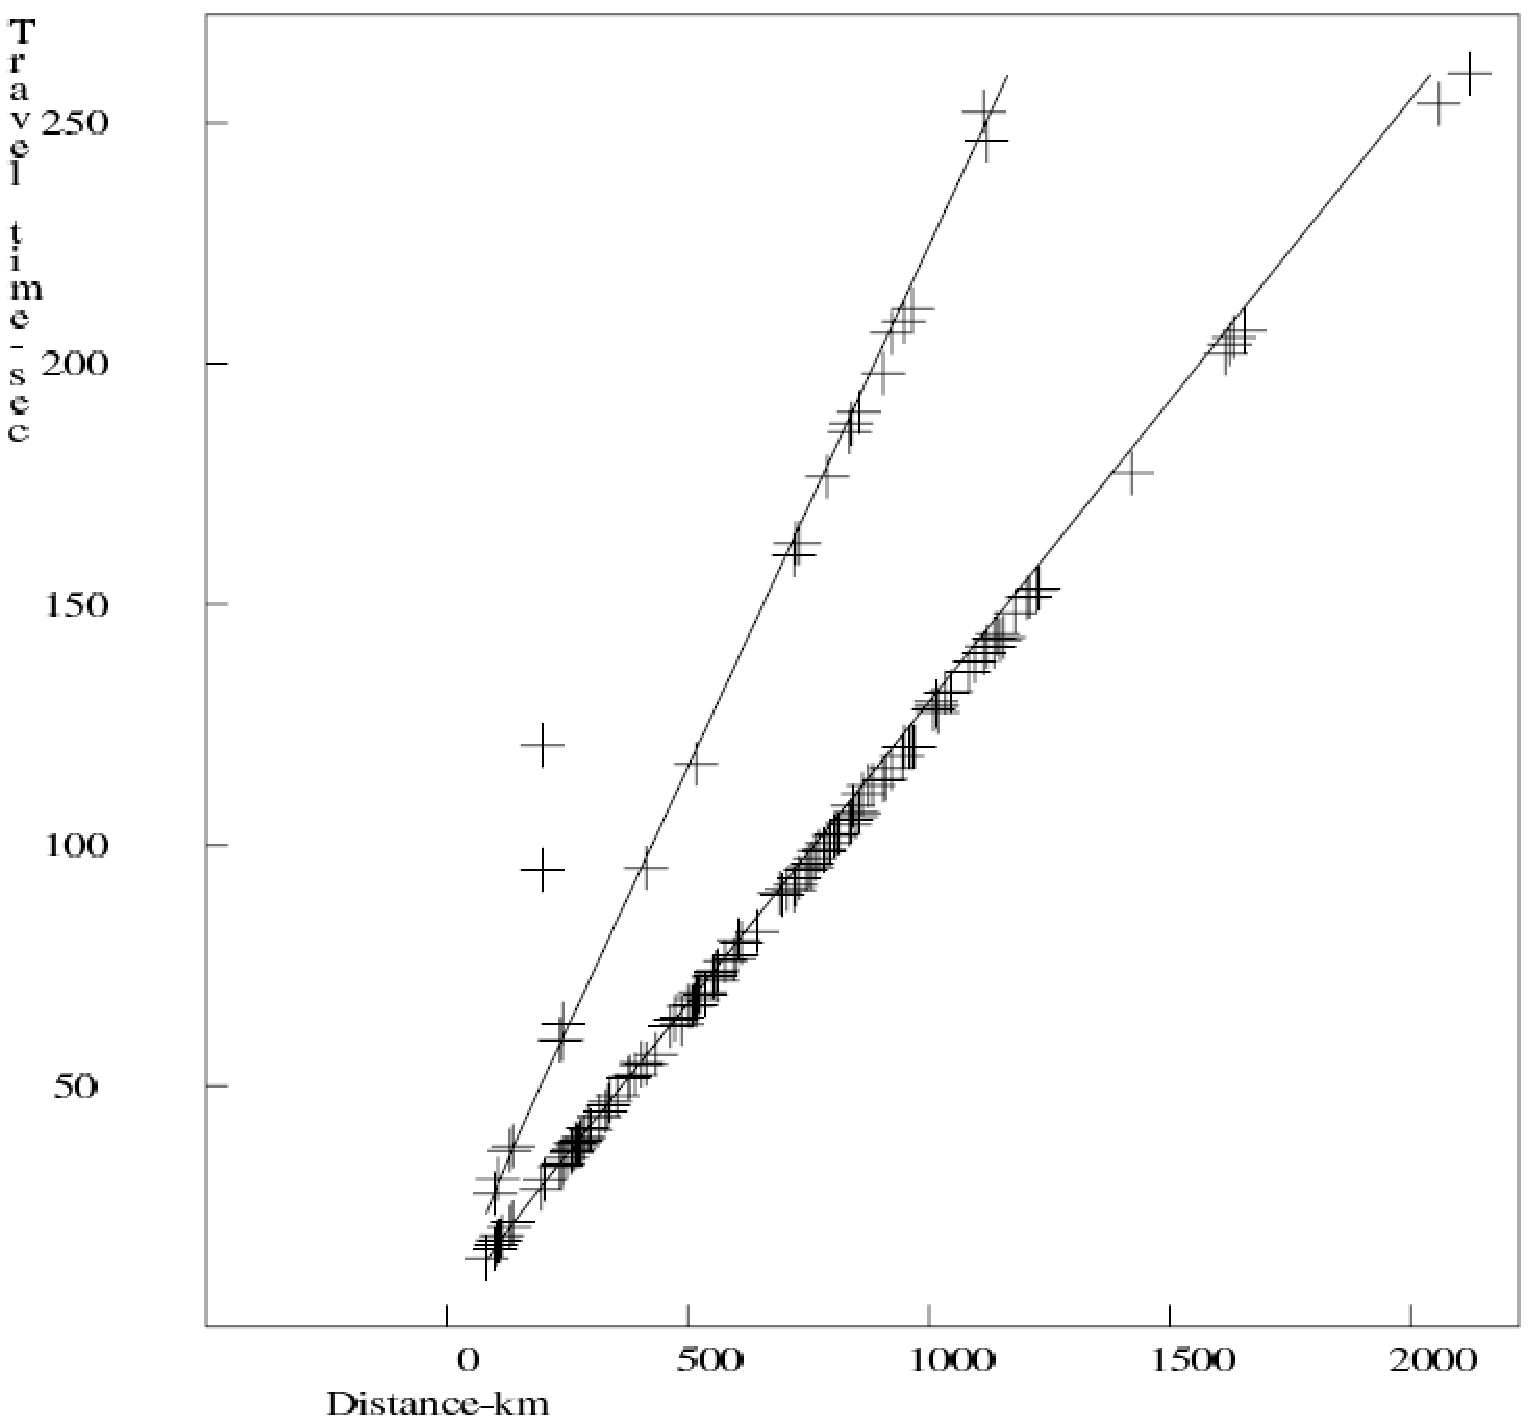
\includegraphics[width=0.9\linewidth]{fig/travel-time-plot}}
\caption{Example of travel time plot. Both P and S observed travel times are plotted with "+"
symbol. Calculated times are shown by the solid lines, the lower one gives the first P arrivals,
the upper line gives first S arrivals. The two outliers are observations from a station with
incorrect timing.
}
\label{fig:travel-time-plot}
\end{figure}


